\documentclass[a4paper, 12pt]{article}
\usepackage[T1]{fontenc}
\usepackage[portuguese]{babel}
\usepackage[utf8]{inputenc}
\usepackage[margin=2cm,includefoot,footskip=30pt,]{geometry}

\usepackage{graphicx}
\graphicspath{ {imagens/} }
\usepackage{bold-extra}
\usepackage{epstopdf}
\usepackage{float}
\usepackage{scalerel}
\usepackage{mathtools}
\usepackage{enumerate}
\usepackage{indentfirst}
\newcommand\showdiv[1]{\overline{\smash{\hstretch{.5}{)}\mkern-3.2mu\hstretch{.5}{)}}#1}}
\newcommand\ph[1]{\textcolor{white}{#1}}


% ----- Cabeçalho e rodapé -----
\usepackage{fancyhdr}
\pagestyle{fancy}
\fancyhf{}

\renewcommand{\headrulewidth}{1pt}
\renewcommand{\footrulewidth}{0.5pt}

\rhead{1º Trabalho Computacional}
\lhead{Matematica Computacional\rightmark}
\rfoot{Página \thepage}
\lfoot{\small Engenharia Electrotécnica e de Computadores - IST}


\usepackage{pdfpages}

\begin{document}

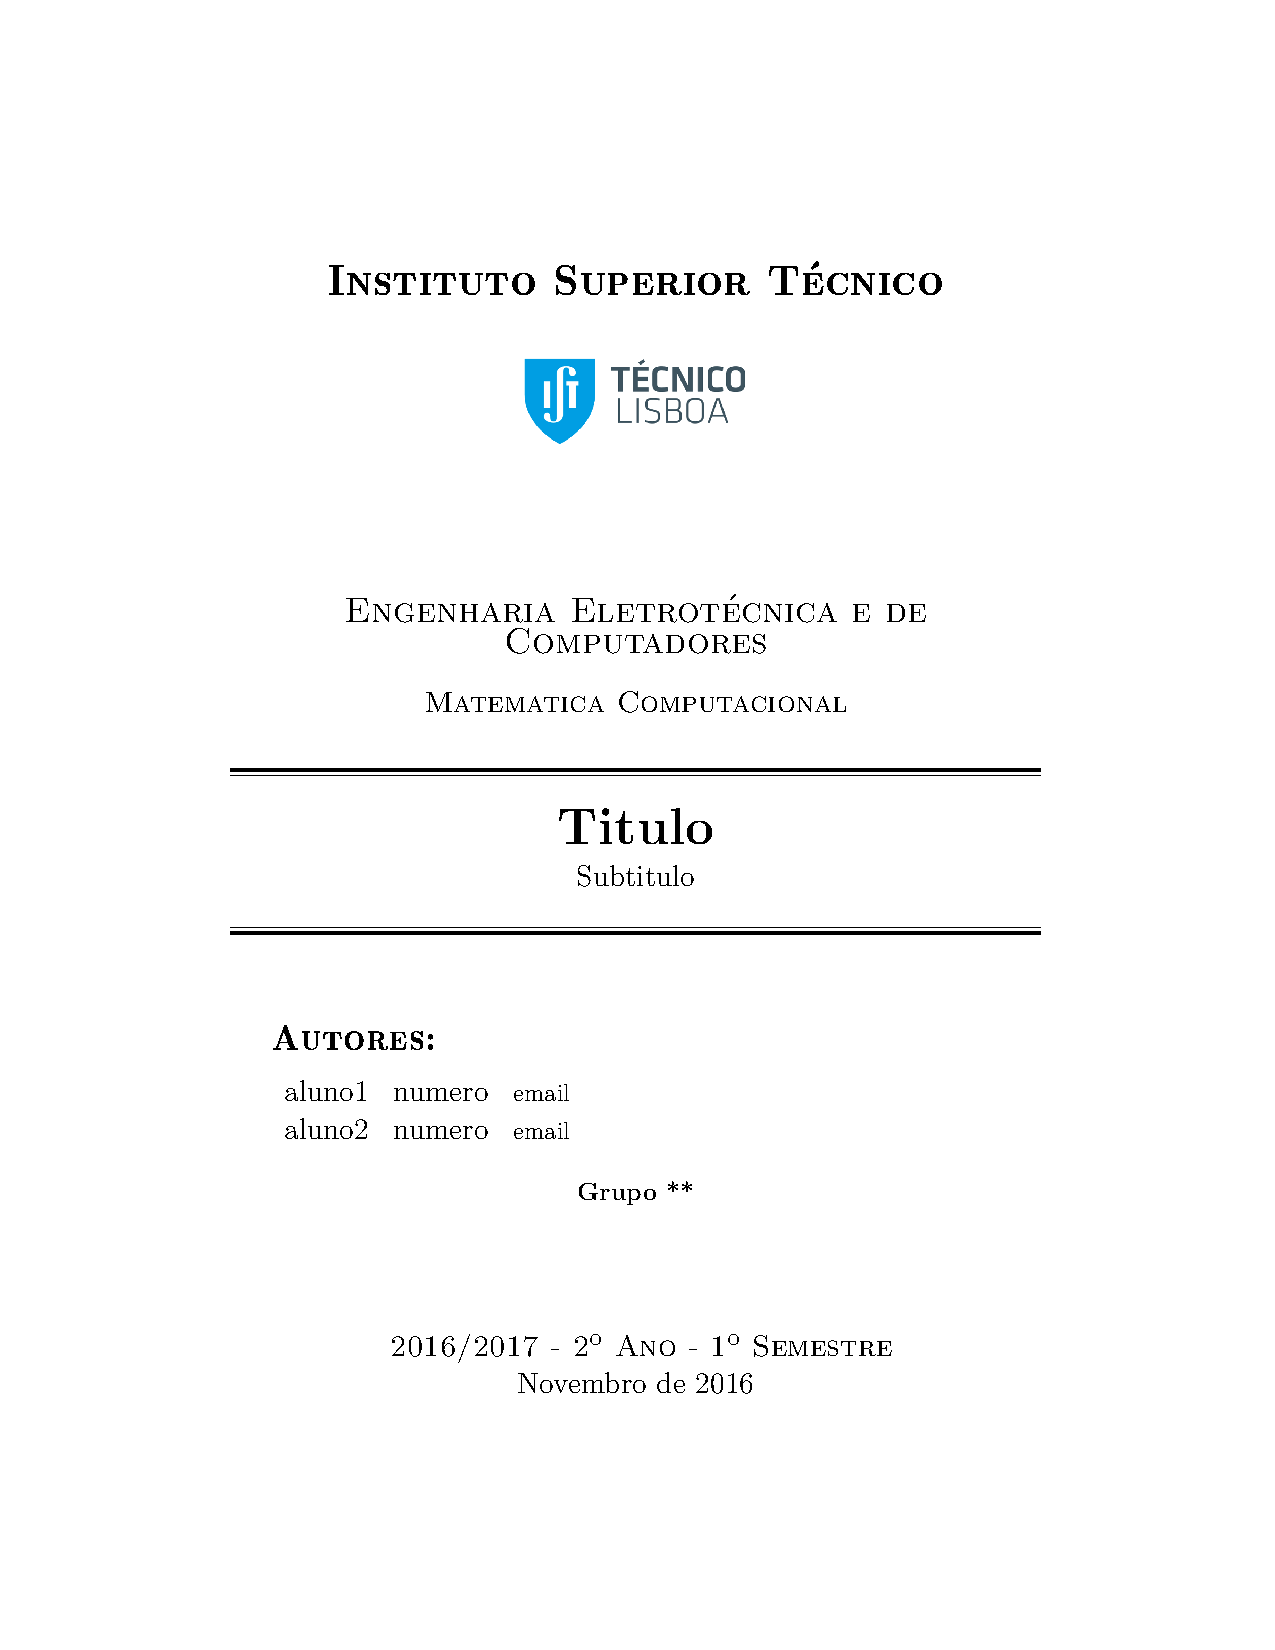
\includepdf[pages={1}]{capa/capa.pdf}

\section{Pergunta 1}
	\begin{equation}
		h(\lambda) = \lambda + 15.5 - 2\cosh(\lambda\tau)
	\end{equation}

	\begin{equation}
		h'(\lambda) = 1 - 2\sinh(\tau\lambda) = 1 - \tau(e^{\tau\lambda} - e^{-\tau\lambda})
	\end{equation}

	\begin{equation}
		h''(\lambda) = -2\tau^2\cosh(\tau\lambda) = -\tau^2(e^{\tau\lambda} + e^{-\tau\lambda})
	\end{equation}

	\par
	Analisemos o sinal de $h''(\lambda)$:
	\begin{equation}
		e^{\tau\lambda} + e^{-\tau\lambda} > 0 \implies h''(\lambda) < 0
	\end{equation}

	\par
	Pelo Teorema de Rolle e pela inequação (4) podemos afirmar que
	$h(\lambda)$ tem no máximo duas raízes. Provemos que $h(\lambda)$ tem no mínimo duas raízes, dado um $\tau$ qualquer.

	\begin{equation}
		h(0) = 0 + 15.5 - 2\cosh(0\tau) = 13.5 > 0
	\end{equation}

	\begin{equation}
	\begin{split}
		\lim_{x \to +\infty} h(\lambda)
		&= \lim_{x \to +\infty} (\lambda + 15.5 - 2\cosh(\lambda)) \\
		&= \lim_{x \to +\infty} e^{\tau\lambda} \bigg(\frac{\lambda}{e^{\tau\lambda}} + \frac{15.5}{e^{\tau\lambda}} - \frac{2\cosh(\lambda)}{e^{\tau\lambda}}\bigg) \\
		&= e^{+\infty} (0 + 0 - 1) = -\infty
	\end{split}
	\end{equation}

	\par
	Analogamente para  $-\infty$ :

	\begin{equation}
	\begin{split}
		\lim_{x \to -\infty} h(\lambda)
		&= \lim_{x \to -\infty} (\lambda + 15.5 - 2\cosh(\lambda)) \\
		&= \lim_{x \to -\infty} e^{-\tau\lambda} \bigg(\frac{\lambda}{e^{-\tau\lambda}} + \frac{15.5}{e^{-\tau\lambda}} - \frac{2\cosh(\lambda)}{e^{-\tau\lambda}}\bigg) \\
		&= e^{+\infty} (0 + 0 - 1) = -\infty
	\end{split}
	\end{equation}

	\par
	Assim, como $h(\lambda)$ é contínua, pelo teoreoma de Bolzano conclui-se que $h(\lambda)$ tem no mínimo duas raízes, uma positiva e uma negativa. Logo, $h(\lambda)$ tem exatamente duas raízes.
	\par
	Se $\tau = 0$, $h(\lambda)$ fica $\lambda + 13,5 = 0 \Leftrightarrow h = -13.5$ . Por outro lado se $\tau$ for muito grande, existirá sempre um $\lambda$ arbritariamente perto de $0^-$ tal que $15.5 = -2cosh(\lambda\tau)$. Assim, a raiz negativa estará contida no intervalo $]-13.5, 0[$.

\section{Pergunta 2}
\subsection*{a)}
\subsection*{b)}
\subsection*{c)}
	Programa em anexo.
\subsection*{d)}
\subsection*{e)}
\subsubsection*{i.)}
\subsubsection*{ii.)}
\subsection*{f)}

\section{Pergunta 3}

\section{Pergunta 4}

\section{Anexo}

\end{document}
